\section{Traffic Differentiation with CSMA/ECA}\label{section3}
Carrier Sense Multiple Access with Enhanced Collision Avoidance~\cite{sanabria2014high, research2standards} is able to build collision-free schedules by using a deterministic backoff after successful transmissions. That is, if all saturated contenders are able to perform a successful transmission and then pick a deterministic backoff, they will not collide among each other in future transmissions.

	\begin{figure*}[tb]
	\centering
		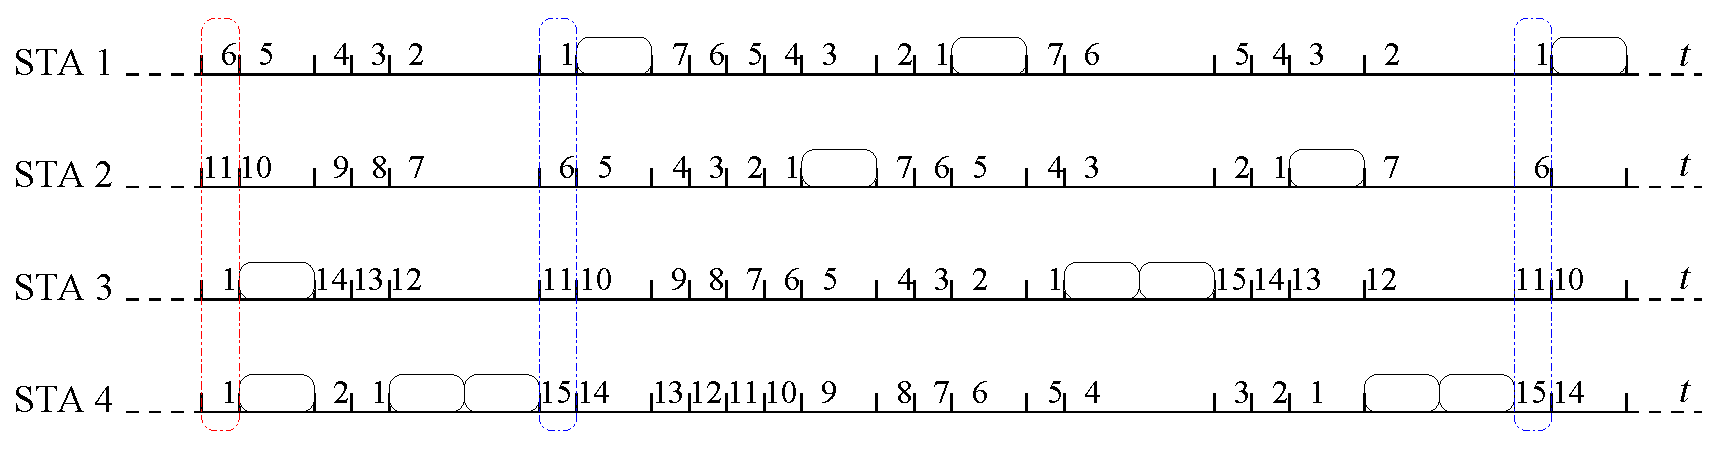
\includegraphics[width=0.8\linewidth]{figures/csma_eca_different_backoff_short.eps}
		\caption{An example of the temporal evolution of CSMA/ECA in saturation}
		\label{fig:ECA}
	\end{figure*}
	
To attempt a transmission, stations generate a random backoff $B\leftarrow\mathcal{U}[0,CW_{\min}-1]$, just as in DCF. Every passing empty slot decrements $B$ in one. When $B=0$, the station will attempt a transmission. If the transmission fails, the node will increment its backoff stage $k\in[0,m]$ in one (where $m$ is the maximum backoff stage of typical value $m=5$) and use another random backoff $B\leftarrow\mathcal{U}[0,CW(k)-1]$; where $CW(k)=2^{k}CW_{\min}$ is the contention window at backoff stage $k$. Otherwise, the successful station will then pick a deterministic backoff for its next transmission, $B_{\text{d}}\leftarrow \lceil CW_{\min}/2\rceil-1$. This value of $B_{\text{d}}$ is roughly equal to the expectation of a random backoff at the same backoff stage ($k=0$, in this case), making it fair and compatible with CSMA/CA stations~\cite{research2standards}.

CSMA/ECA is also capable of allocating many contenders in a collision-free schedule by not reseting the backoff stage $k$ after a successful transmission, as opposed to CSMA/CA. That is, a node at backoff stage $k$ would select $B_{\text{d}}\leftarrow \lceil CW(k)/2\rceil-1$ as its deterministic backoff after a successful transmission. This extension to CSMA/ECA is called Hysteresis. 

Hysteresis forces some contenders to have larger schedules than others, resulting in an unfair distribution of the network resources. This effect can be compensated by allowing nodes at backoff stage $k$ to transmit $2^{k}$ packets upon each transmission attempt. We call this extension Fair Share and it ensures an even distribution of the available throughput among contenders.

Figure~\ref{fig:ECA} shows a temporal example of CSMA/ECA with its extensions, namely, Hysteresis and Fair Share~\cite{sanabria2014high}. The \emph{STA-\#} labels denote the saturated contenders. The horizontal lines represent time, where the numbers are the number of empty slots left until the expiration of the backoff counter. In the figure, the first outline indicates a collision which forces STA-3 and STA-4 to increase their backoff stages ($k \leftarrow \min(k+1,m)$) and use a random backoff, $B\leftarrow\mathcal{U}[0,CW(k)-1]$. When STA-4's backoff expires, it will then transmit $2^{k}$ packets. Because the transmission was successful it uses $B_{\text{d}}=\lceil CW(k)/2\rceil-1$ as its deterministic backoff for the next transmission. Notice that once all stations transmit successfully collisions are eliminated.

CSMA/ECA with Hysteresis and Fair Share (CSMA/ECA$_{\text{Hys+FS}}$) is able to outperform CSMA/CA, as shown in the simulation results presented in Figures~\ref{fig:CAvsECA} and~\ref{fig:col-CAvsECA}. For the sake of clarity, Algorithm~\ref{alg:DCF} and Algorithm~\ref{alg:ECA} exemplify CSMA/CA and CSMA/ECA$_{\text{Hys+FS}}$ respectively.

	\begin{figure}[tb]
	\centering
		\includegraphics[width=0.7\linewidth, angle=-90]{figures/throughput-perfectChannel.eps}
		\caption{Average aggregated throughput ($CW_{\min}=32$)\cite{sanabria2014high}}
		\label{fig:CAvsECA}
	\end{figure}
	
	\begin{figure}[tb]
	\centering
		\includegraphics[width=0.7\linewidth, angle=-90]{figures/collisions-perfectChannel.eps}
		\caption{Average aggregated number of collision slots ($CW_{\min}=32$)\cite{sanabria2014high}}
		\label{fig:col-CAvsECA}
	\end{figure}

	\begin{algorithm}[t]
	\While{the device is on}
	{
	  %\tcc{Initialize retransmission attempts.}
	  $r \leftarrow 0$; $k \leftarrow 0$\;
	  %\tcc{Initialize backoff counter.}
	  $B \leftarrow \mathcal{U}[0,2^k{\rm{CW}_{min}}-1]$\;
	  \While{there is a packet to transmit}{
	    %\tcc{Initialize $a$.}
	    \Repeat{($r = R$) or (success)}{
	      %\tcc{First, backoff.}
	      \While{$B>0$}{
	        wait 1 slot\;
	        $B \leftarrow B-1$\;
	      }
	      \colorbox{yellow}{Attempt transmission of 1 packet;}\\
	      \If{collision}{\label{collision}
	        %\tcc{Random backoff.}
	        $r \leftarrow r+1$\;
	        $k \leftarrow \min (k+1,m)$\;
	        $B \leftarrow \mathcal{U}[0, 2^k {\rm{CW}_{min}} -1]$\;\label{finalCollision}
	      }
	    }
	    $r \leftarrow 0$\;
	    \colorbox{yellow}{$k \leftarrow 0$;}\\
		 \eIf{success}{
	      %\tcc{Random backoff.}
	      \colorbox{yellow}{$B \leftarrow \mathcal{U}[0,2^{k}{\rm{CW}_{min}}-1]$;}\\\label{randomBackoff}
	    }
	    {
	      Discard packet\;
	      $B \leftarrow \mathcal{U}[0,2^k {\rm{CW}_{min}}-1]$\;
	    }
	  }
	  Wait until there is a packet to transmit\;
	}
	\caption{\small{CSMA/CA. $r$ indicates the number of retransmission attempts, while $R$ is the maximum retransmission attempts limit. When it is reached, the packet waiting for transmission is dropped.}}
	\label{alg:DCF}
	\end{algorithm}

	\begin{algorithm}[t]
	\While{the device is on}
	{
	  $r \leftarrow 0$ ; $k \leftarrow 0$ ; $k_{c} \leftarrow k$\;
	  $b \leftarrow \mathcal{U}[0,2^k\rm{CW}_{min}-1]$\;
	  \While{there is a packet to transmit}{
	    %\tcc{Initialize $a$.}
	    \Repeat{($r = R$) or (success)}{
	      %\tcc{First, backoff.}
	      \While{$B>0$}{
	        wait 1 slot\;
	        $B \leftarrow B-1$\;
	      }
	      \colorbox{yellow}{Attempt transmission of $2^k$ packets;}\\
	      \If{collision}{
	        %\tcc{Random backoff.}
	        $r \leftarrow r+1$\;
	        $k \leftarrow \min (k+1,m)$\;
	        $B \leftarrow \mathcal{U}[0, 2^k  \rm{CW}_{min} -1]$\;
	      }
	    }
	    $r \leftarrow 0$\;
	    %$s \leftarrow 0$\;
	    \eIf{success}{
	      %\tcc{Random backoff.}
	      \colorbox{yellow}{$B_{d} \leftarrow \lceil 2^{k}\rm{CW}_{min}/2\rceil-1$;}\label{deterministicBackoff}\\
		$B \leftarrow B_{d}$\;
	    }
	    {
	      Discard $2^{k_{c}}$ packets\label{discard}\;
%	      $k \leftarrow 0$\;
	      $B \leftarrow \mathcal{U}[0, 2^k \rm{CW}_{min}-1]$\;
	    }
	
	$k_{c} \leftarrow k$\;
	  }
	  Wait until there is a packet to transmit\;
	}	
	\vspace{0.2cm}
	\caption{CSMA/ECA$_{\text{Hys+FS}}$: $k_{c}$ refers to the contention backoff stage, that is, the backoff stage with which a contention for transmission is started. After $R$ retransmission attempts, Fair Share instructs the node to drop $2^{k_{c}}$ packets}
	\label{alg:ECA}
	\end{algorithm}
	
%	\begin{algorithm}[tb]
%	\While{the device is on}
%	{
%	  $r \leftarrow 0$ ; $k \leftarrow 0$\;
%	  $b \leftarrow \mathcal{U}[0,2^k\rm{CW}_{min}-1]$\;
%	  \While{there is a packet to transmit}{
%	    %\tcc{Initialize $a$.}
%	    \Repeat{($r = R$) or (success)}{
%	      %\tcc{First, backoff.}
%	      \While{$B>0$}{
%	        wait 1 slot\;
%	        $B \leftarrow B-1$\;
%	      }
%	      \colorbox{yellow}{Attempt transmission of $2^k$ packets;}\\
%	      \If{collision}{
%	        %\tcc{Random backoff.}
%	        $r \leftarrow r+1$\;
%	        $k \leftarrow \min (k+1,m)$\;
%	        $B \leftarrow \mathcal{U}[0, 2^k  \rm{CW}_{min} -1]$\;
%	      }
%	    }
%	    $r \leftarrow 0$\;
%	    %$s \leftarrow 0$\;
%	    \eIf{success}{
%	      %\tcc{Random backoff.}
%	      \colorbox{yellow}{$B_{\text{d}} \leftarrow (2^{k}\rm{CW}_{min})/2-1$;}\\\label{deterministicBackoff}
%		$B \leftarrow B_{\text{d}}$;\\
%	    }
%	    {
%	      Discard packet\;
%	       \colorbox{yellow}{$k \leftarrow 0$}\label{eca:stageReset}\;
%	      $B \leftarrow \mathcal{U}[0, 2^k \rm{CW}_{min}-1]$\;
%	    }
%	  }
%	  Wait until there is a packet to transmit\;
%	}
%	\vspace{0.2cm}
%	\caption{CSMA/ECA$_{\text{Hys+FS}}$}
%	\label{alg:ECA}
%	\end{algorithm}

The main difference between Algorithm~\ref{alg:DCF} and Algorithm~\ref{alg:ECA}, and therefore between CSMA/CA and CSMA/ECA$_{\text{Hys+FS}}$ is that the latter uses a deterministic backoff after a successful transmission. This difference is highlighted at line~\ref{randomBackoff} and line~\ref{deterministicBackoff} of Algorithms~\ref{alg:DCF} and~\ref{alg:ECA}, respectively.

\subsection{Schedule Reset mechanism}\label{scheduleReset}
CSMA/ECA$_{\text{Hys+FS}}$ instructs nodes not to reset their backoff stage after a successful transmission. This is done in order to increase the cycle length and provide a collision-free schedule for many contenders, which is desirable in dense scenarios.

%The increment of the backoff stage and consequently the enlargement of the deterministic backoff are the result of previous collisions. In WLANs, collisions are assumed when the transmitter does not receive an Acknowledgement (ACK) packet from the receiver after a SIFS period following the transmission of the data frame. This means that channel imperfections preventing the reception of ACKs would be assumed as collisions by the senders, therefore, will also provoke an increase on the deterministic backoff in CSMA/ECA$_{\text{Hys+FS}}$.

Having a big deterministic backoff increases the time between successful transmissions. Furthermore, if not operating in a scenario with many nodes the empty slots between transmissions are not longer negligible and degrade the overall throughput of the system. For instance, if nodes withdraw from the contention their previously used slots will now be empty. Contenders should be aware of this issue and pursue opportunities to reduce their deterministic backoff without sacrificing too much in collisions. 

The \emph{Schedule Reset} mechanism for CSMA/ECA$_{\text{Hys+FS}}$ introduced in~\cite{sanabria2014high} consists on finding the smallest collision-free schedule between a contender's transmissions and then change the node's deterministic backoff to fit in that schedule. Take a contender with a $B_{\text{d}}=31$ as an example. By listening to the slots between its transmissions, we are able to determine the availability of smaller (and possibly) collision-free schedules. 

Figure~\ref{fig:scheduleReset1} shows the slots between the transmissions of a contender with $B_{\text{d}}=31$. Starting from the left, the current $B_{\text{d}}=0$ means that the slot will be filled with the contender's own transmission. Each following slot containing either a transmission or a collision is identified with the number one, while empty slots are marked with a zero. Notice that the highlighted empty slots appear every eight slots, suggesting that a schedule reduction from $B_{\text{d}}=31$ to $B_{\text{d}}^{*}=7$ is possible. The schedule change is performed after the contender's next successful transmission. 

%coupled with an increase by one in the node's \emph{stickiness}~\cite{L_MAC2}. 

%\footnote{Trailing waiting periods, like the SIFS, are composed of empty slots. These allow nodes to decrement their backoff counters even after a collision or successful slots. Without loss of generality, the stations in our examples and simulations decrement their respective backoff counters by one after these kind of slots (see example in Figures~\ref{fig:ECA} and~\ref{fig:ecaQoS}).}

	\begin{figure}[tb]
	\centering
		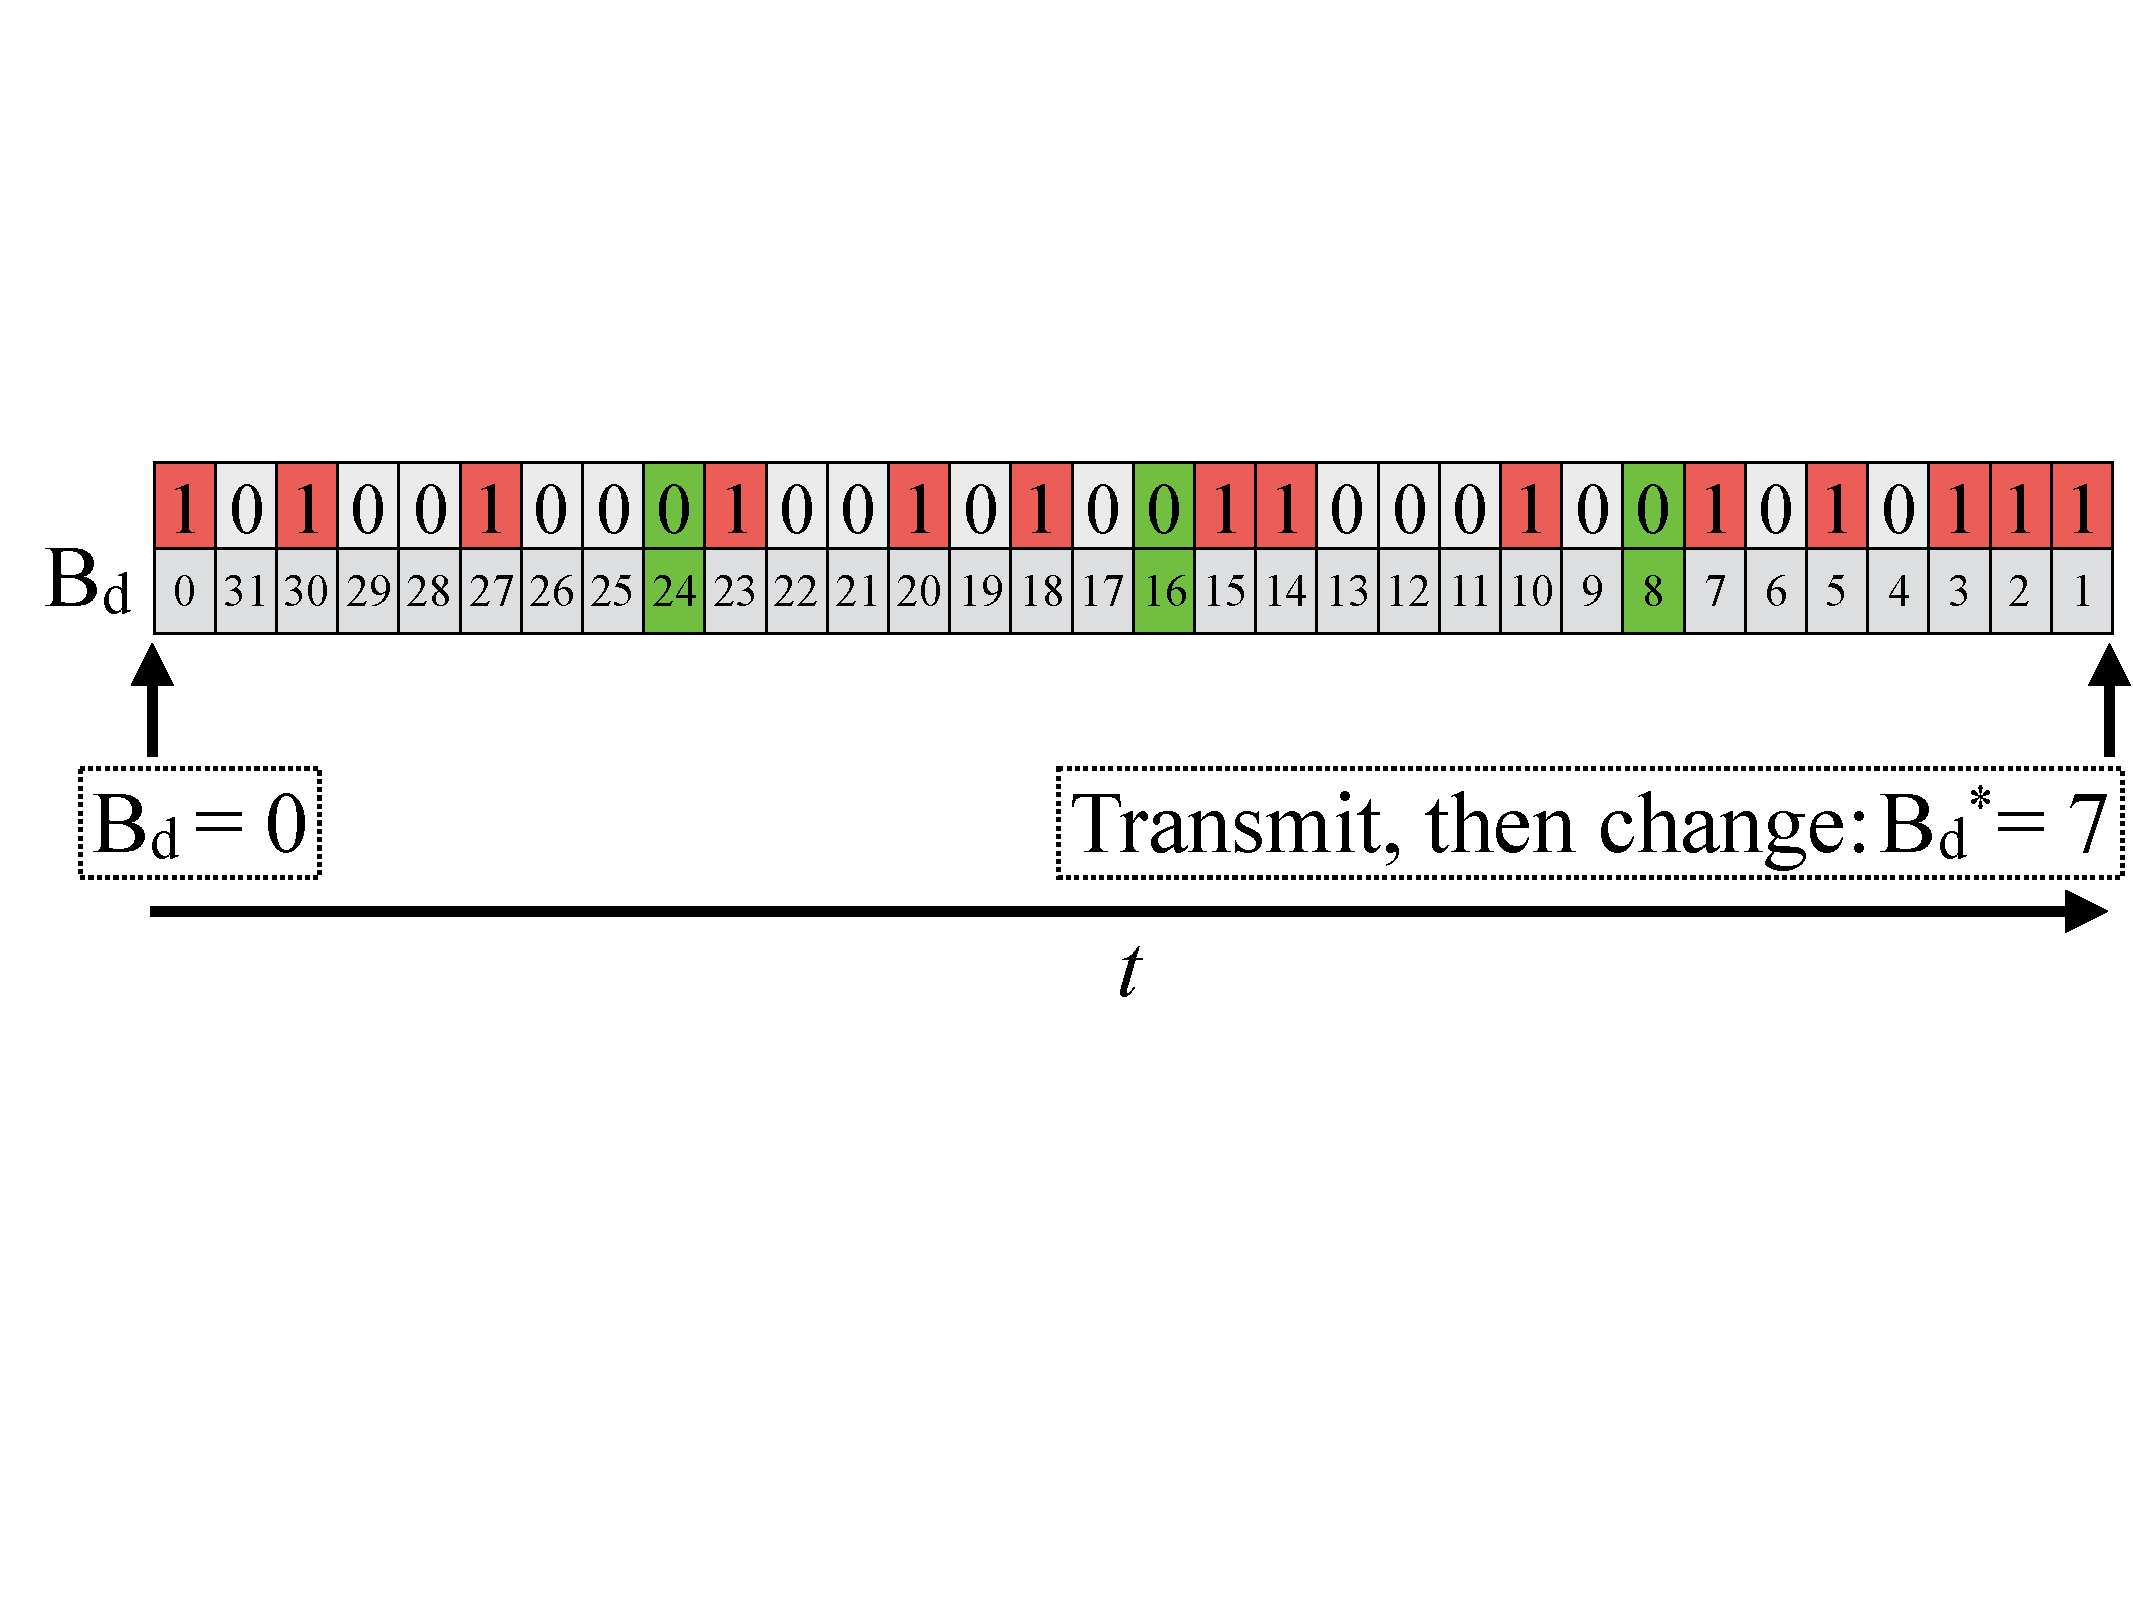
\includegraphics[width=\linewidth]{figures/scheduleReset.pdf}
		\caption{Example of the Schedule Reset mechanism (extracted from~\cite{sanabria2014high})}
		\label{fig:scheduleReset1}
	\end{figure}

Schedule Reset (SR) is implemented in CSMA/ECA$_{\text{Hys+FS}}$ by filling a bitmap $b$ of size $B_{\text{d}}+1$. Each bit $t,~t\in\{0,\ldots ,B_{\text{d}}\}$ in the bitmap is the result of a bitwise OR operation between its current value, $b[t]$ and the state of the slot; which equals to one when busy or zero when idle. After $\gamma$ consecutive successful transmissions (sxTx), the bitmap is evaluated. If a change of schedule is possible, it is executed just after the next successful transmission.

It is possible to configure Schedule Reset in two modes, namely \emph{conservative} and \emph{aggressive}. These modes relate to the number of consecutive transmissions needed to evaluate the bitmap, that is, $\gamma$. A conservative SR contains the information of all users' transmissions, therefore no additional collisions are introduced as a consequence of the schedule change. This implies a value of $\gamma=2^{m-1}CW_{\min}/B_{\text{d}}$. On the other hand, setting $\gamma=1$ triggers a bitmap evaluation after just two consecutive transmissions, rendering this choice of $\gamma$ the aggressive mode.

Aggressive Schedule Reset coupled with an increase in the Stickiness has proven to be suitable for noisy scenarios~\cite{sanabria2014high}. Stickiness is not a new concept to CSMA/ECA~\cite{barcelo2011tcf}. It simply instructs the contender to \emph{stick} to the deterministic backoff even in the event of \emph{stickiness} number of failed transmissions. This allows for a faster convergence towards a collision-free schedule. CSMA/ECA$_{\text{QoS}}$ with a default level of stickiness equal to $2$ has proven to provide the better combination of high throughput and low collisions, as shown in Figure~\ref{fig:stickEv-throughput-overallOnly}. 

\begin{figure}[tb]
	\centering
		\includegraphics[width=0.7\linewidth, angle=-90]{figures/stickEv-throughput-overallOnly.eps}
		\caption{Average throughput and collisions with different levels of stickiness for CSMA/ECA$_{\text{QoS}}$ in non-saturation conditions (as explained in Section~\ref{subsect:simParams})}
		\label{fig:stickEv-throughput-overallOnly}
	\end{figure}

%The Schedule Reset mechanism is activated after a complete schedule with a deterministic backoff, that is, the contender has performed $B_{d}/C$ successful transmissions, where $C$ is the number of slots in a complete schedule (like the exemplified in Section~\ref{ECAqosCollisionFree}).

\subsection{Incorporating multiple ACs into CSMA/ECA}
As shown before, CSMA/ECA and its extensions (referred to as CSMA/ECA$_{\text{Hys+FS}}$ from this point forward) are able to construct a collision-free schedule under saturated conditions, outperforming CSMA/CA. Furthermore, CSMA/ECA$_{\text{Hys+FS}}$ uses the same default contention parameters used by CSMA/CA, so the compatibility is maintained~\cite{sanabria2014high}.

Providing priority is to ensure a more frequent access to some ACs over others. In CSMA/ECA$_{\text{Hys+FS}}$ this is only subject to the deterministic backoff. That is, an AC using a shorter $B_{\text{d}}$ would in turn access the channel more often than those using a larger one. To maintain compatibility with EDCA, CSMA/ECA$_{\text{Hys+FS}}$ considers the same four ACs and CW values shown in Table~\ref{tab:EDCAparams}. 

Nevertheless, AIFS and TXOP are not fit for multiple CSMA/ECA$_{\text{Hys+FS}}$ queues. For instance, AIFS values are not required since differentiation is only provided by the deterministic backoff. The incorporation of different AIFS for each category would trigger Virtual Collisions that in turn may disrupt an existent collision-free schedule. Figure~\ref{fig:AIFSinECA} shows a VC in CSMA/ECA$_{\text{Hys+FS}}$ (indicated by the outline) consequence of using AIFS during a collision-free schedule.

	\begin{figure}[tb]
	\centering
		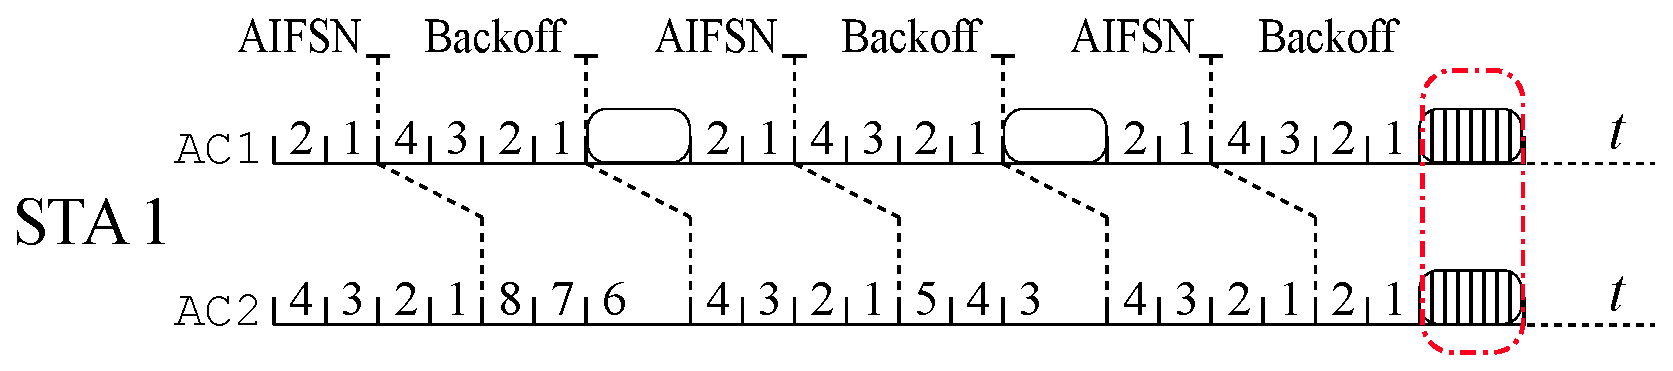
\includegraphics[width=\linewidth]{figures/AIFSwithECA.eps}
		\caption{Example temporal evolution of CSMA/ECA$_{\text{Hys+FS}}$ with two ACs using AIFS resulting in a virtual collision. Only considering AIFSN values of 2 and 4, $B_{\text{d}}$ of 4 and 8 for AC1 and AC2 respectively}
		\label{fig:AIFSinECA}
	\end{figure}


TXOP in EDCA ensures that all traffic from the same category receives on average the same channel time rather than the same throughput. In contrast, CSMA/ECA$_{\text{Hys+FS}}$'s goal through Fair Share is to provide close to equal average throughput to same-priority ACs. We leave the elaboration of an adaptive Fair Share which ensures resource fairness rather than throughput fairness as a future research topic.
%Nevertheless, this can be misleading. Take two low same-priority ACs, if using different transmission rates it will take different periods of time to complete each transmission. This defies the purpose of TXOP given that the network resources are not evenly shared. 

As EDCA extends DCF into four ACs, similarly there is an instance of CSMA/ECA$_{\text{Hys+FS}}$ for each AC. We will refer to CSMA/ECA$_{\text{Hys+FS}}$ with multiple ACs as CSMA/ECA$_{\text{QoS}}$ from here forward. Table~\ref{tab:ecaQosParams} shows the CW as well as the lowest and largest $B_{\text{d}}$ for ACs in CSMA/ECA$_{\text{QoS}}$.

Figure~\ref{fig:ecaQoS} shows an example of CSMA/ECA$_{\text{QoS}}$ with two contenders and two ACs; where AC1 has higher priority than AC2. In the figure, the first outline indicates a VC between AC1 and AC2 from STA-2. VC in CSMA/ECA$_{\text{QoS}}$ are handled just as in EDCA, that is, the AC with the highest priority is granted access to the channel, while the other ACs involved in the VC double their contention windows and use a random backoff for the next transmission. Consequently, AC1 from STA-2 successfully transmits and then uses $B_{\text{d}}=\frac{2^{0}CW_{\min}[\text{AC1}]}{2}-1= 3$.

Still on Figure~\ref{fig:ecaQoS}, the second outline indicates a collision between STA-2's AC2 and AC1 from STA-1. At this moment in time STA-2 AC2's backoff stage has been increased in two occasions ($k[\text{AC2}]=2$). When said AC2 is able to transmit, it sends $2^{k[\text{AC2}]}$ packets according to Fair Share. Then, it uses a deterministic backoff, $B_{\text{d}}=\frac{2^{k[\text{AC2}]}CW_{\min}[\text{AC2}]}{2}-1=31$.

	\begin{figure*}[tb]
	\centering
		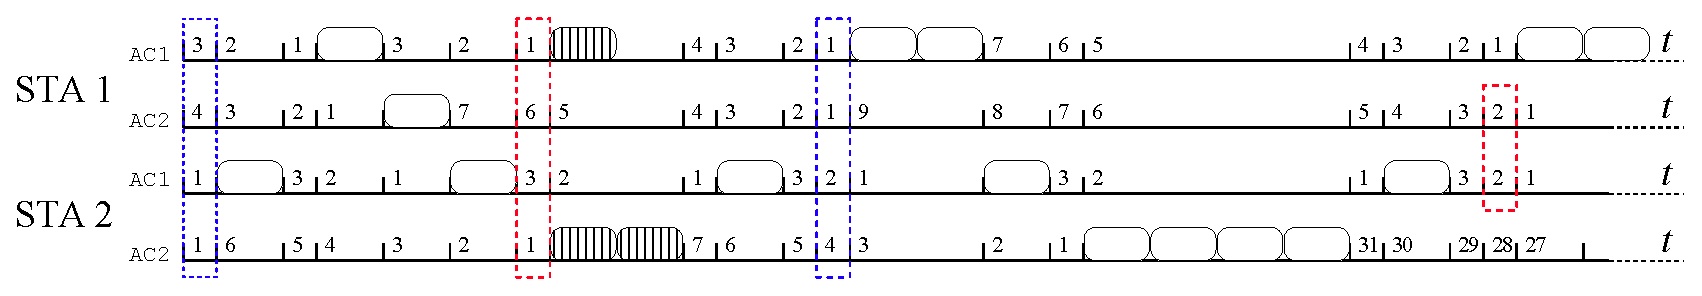
\includegraphics[width=0.9\linewidth]{figures/csma-eca-hew-oldScheme-fixed.eps}
		\caption{An example of the temporal evolution of CSMA/ECA$_{\text{QoS}}$ in saturation ($CW_{\min}[\text{AC1,AC2}]=[8,16]$; $m[\text{AC1,AC2}]=[5,5]$)}
		\label{fig:ecaQoS}
	\end{figure*}

The third outline in Figure~\ref{fig:ecaQoS} indicates an VC in STA-1, which is resolved allowing AC1 and deferring AC2's transmission using a random backoff with a doubled CW. A future collision between STA-2's AC1 and AC2 from STA-1 is highlighted by the last outline.

\subsection{Collisions and Virtual Collisions-free operation using Smart Backoff}\label{ECAqosCollisionFree}
Consider a complete schedule of length $C=2^{m}CW_{\min}$, and $m=5$. With CSMA/ECA$_{\text{Hys+FS}}$ and a single AC it is possible to allocate a collision-free transmission slot for up to $C/2=512$ contenders (the highest $B_{\text{d}}+1$ for AC Legacy in Table~\ref{tab:ecaQosParams}). Nevertheless, with CSMA/ECA$_{\text{QoS}}$ and all ACs in saturation each contender mimics the behaviour of four saturated nodes (one for each AC). This means that the total number of supported collision-free contenders will be reduced in order to provide a transmission slot for all the ACs in the network. If all the ACs are in saturation, i.e., have a packet to transmit, CSMA/ECA$_{\text{QoS}}$ can provide collision-free operation for up to $2^{m[\text{VO}]}CW_{\min}[\text{VO}]/2=8$ contenders, where $m[\text{VO}]$ is the maximum backoff stage of the AC with the smallest $CW_{\max}$. Even-though Table~\ref{tab:ecaQosParams} provides CSMA/ECA$_{\text{QoS}}$'s default contention parameters, these will be adjusted in Section~\ref{sim:results} in order to support more contenders while in saturation.

VCs in CSMA/ECA$_{\text{QoS}}$ force ACs to defer their transmissions using a random backoff. Therefore, VCs can disrupt any existent collision-free schedule in CSMA/ECA$_{\text{QoS}}$, wasting channel time recovering from collisions and degrading the overall throughput. Given that all AC's backoff counters are known to the contender, there is nothing preventing it from using this information to avoid future VCs.

CSMA/ECA$_{\text{QoS}}$ eliminates VCs by picking a $B[\text{AC}]$ that is not equal to any of the other AC's counters. This is exemplified in Figure~\ref{fig:smartBackoff1}. The figure shows a contender with four ACs and $B_{\text{d}}[4]=[4,8,16,16]$, for AC1 to AC4 respectively. AC1 effectively transmits, but AC3 suffers from a VC. It then selects a random backoff, $B[\text{AC3}]=24$, which is different from any other AC's counters. Then, to eliminate future VCs in CSMA/ECA$_{\text{QoS}}$ the successes of other ACs's transmissions should also be taken into account. This is achieved by selecting a number whose absolute difference with each of the other AC's counters is not a multiple of each comparison's smallest deterministic backoff. Algorithm~\ref{alg:smartBackoff} shows the process of selecting what is referred to as a \emph{Smart Backoff} in CSMA/ECA$_{\text{QoS}}$. It shows four ACs, although it can used to eliminate VCs with as many ACs as needed. Smart Backoff is used instead of a random backoff in CSMA/ECA$_{\text{QoS}}$.

%Nevertheless, because CSMA/ECA$_{\text{QoS}}$ ACs use a deterministic backoff after successful transmissions the selected $B[\text{AC3}]$ will eventually collide with AC1's next sixth successful transmission.

	\begin{algorithm}[t]
		$AC:=4$\tcp*[l]{number of Access Categories}
		$CW_{\min}[AC]$\tcp*[l]{$CW_{\min}$ for all ACs}
		$B_{\text{d}}[AC]$\tcp*[l]{$B_{\text{d}}$ for all ACs}
		$B[AC]$\tcp*[l]{current $B$ from all ACs}
		$k[AC]$\tcp*[l]{current backoff stage}
		$F[AC]:=\{0\}$\;
		$Cb[AC]:=\{0\}$\;
		\tcp{}\tcp{looking for a suitable $B[i]$; $i\in[1,AC]$}\tcp{}
		\While{$($F$~\neq 1)$ or $($Cb$~\neq 1)$}	
		{
			$B[i]\gets\mathcal{U}[0,2^{k[i]}{CW_{\min}[i]}]$\;
			\For{$(j = 1; j\leq \text{AC};j++)$}
			{
				\If{$(j\neq i)$}{
					$F[j]\gets |B[i]-B[j]|$~mod~$[\min(B_{\text{d}}[i],B_{\text{d}}[j])]$\;
					\If{$(F[j]\neq 0)$} 
					{	
						$F[j]\gets 1$\;
					}
					\eIf{$(B[i]\neq B[j])$}{
						$Cb[j]\gets 1$\;
					}{
						$Cb[j]\gets 0$\;
					}
				}
			}
			
			
		}
		\Return $(B[i])$\;
		\vspace{0.2cm}
		\caption{Smart Backoff: eliminating Virtual Collisions in CSMA/ECA$_{\text{QoS}}$}
		\label{alg:smartBackoff}
	\end{algorithm}

What results from Algorithm~\ref{alg:smartBackoff} is a Smart Backoff counter that will not cause a VC on the next transmission attempts while in saturation.

	\begin{table}[tb]
		\centering
		\caption{Deafult CSMA/ECA$_{\text{QoS}}$ contention parameters}
		\label{tab:ecaQosParams}
		\begin{tabular}{|c|c|c|c|c|c|}
			\hline
			{\bfseries AC} & {\bfseries CW$_{\min}$} & {\bfseries CW$_{\max}$} & {\bfseries m} & {\bfseries lowest $B_{\text{d}}$} & {\bfseries highest $B_{\text{d}}$}\\
			\hline
			BK		       &	32				&		1024		  & 		5	&			15		        &		511\\
			BE		       &	32				&		1024		  &		5	&			15		        &		511\\
			VI		       &	16				&		32		  & 		1	&			7		        &		15\\
			VO		       &	8				&		16		  & 		1	&			3		        &		7\\
			Legacy	       &	32				&		1024		  & 		5	&			15		        &		511\\
			\hline
		\end{tabular}
	\end{table}

	\begin{figure}[tb]
	\centering
		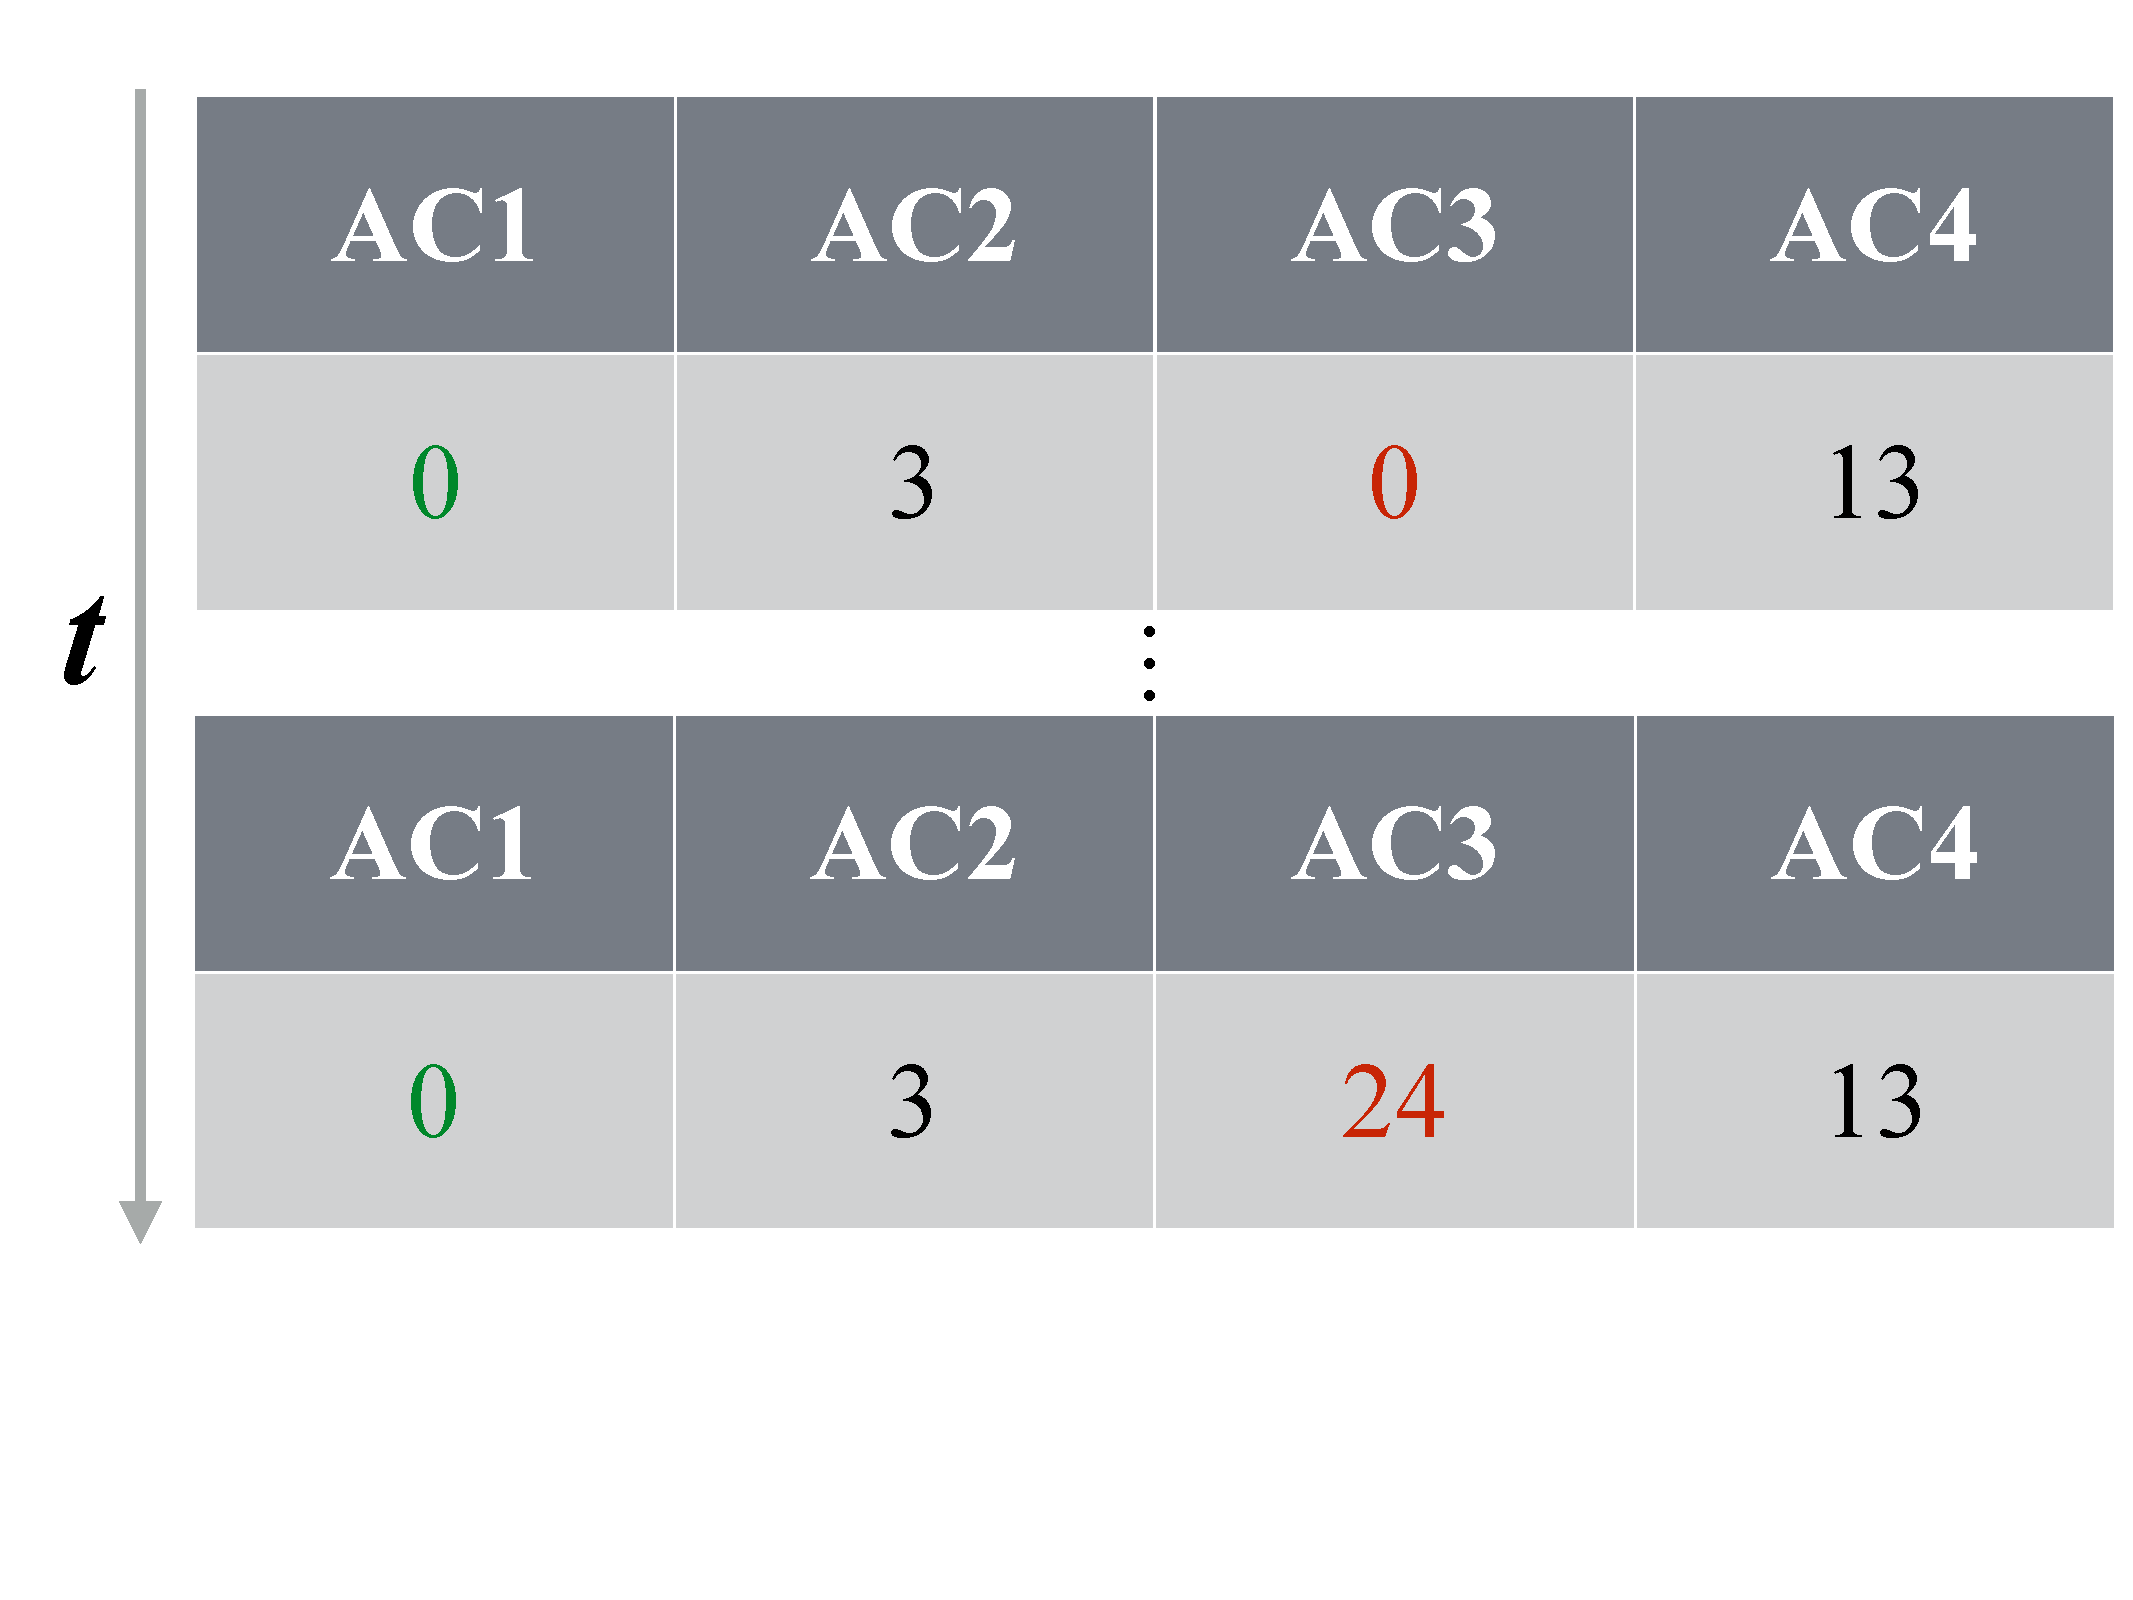
\includegraphics[width=0.8\linewidth]{figures/smartBackoff1.pdf}
		\caption{Four AC backoff counters in a CSMA/ECA$_{\text{QoS}}$ node with $B_{\text{d}}[4]=[4,8,16,16]$. After a VC or collision, the new random backoff counter must not be equal to any other AC's counter}
		\label{fig:smartBackoff1}
	\end{figure}
